\documentclass[12pt]{ociamthesis}  % default square logo 
%\documentclass[12pt,beltcrest]{ociamthesis} % use old belt crest logo
%\documentclass[12pt,shieldcrest]{ociamthesis} % use older shield crest logo

%load any additional packages
\usepackage{amssymb}
\usepackage{listings}
\usepackage{float}
\usepackage{graphicx}
\usepackage{color}
 
\definecolor{codegreen}{rgb}{0,0.6,0}
\definecolor{codegray}{rgb}{0.5,0.5,0.5}
\definecolor{codepurple}{rgb}{0.58,0,0.82}
\definecolor{backcolour}{rgb}{0.95,0.95,0.92}
 
\lstdefinestyle{mystyle}{
    backgroundcolor=\color{backcolour},   
    commentstyle=\color{codegreen},
    keywordstyle=\color{magenta},
    numberstyle=\tiny\color{codegray},
    stringstyle=\color{codepurple},
    basicstyle=\footnotesize,
    breakatwhitespace=false,         
    breaklines=true,                 
    captionpos=b,                    
    keepspaces=true,                 
    numbers=left,                    
    numbersep=5pt,                  
    showspaces=false,                
    showstringspaces=false,
    showtabs=false,                  
    tabsize=2,
    language=python
}
 
\lstset{style=mystyle}

%input macros (i.e. write your own macros file called mymacros.tex 
%and uncomment the next line)
%\include{mymacros}

\title{Tugas Chapter 1 \\[1ex]     %your thesis title,
        Artificial Intelligence}   %note \\[1ex] is a line break in the title

\author{Dyning Aida Batrishya}             %your name
\college{1184030\\[5ex]
D4 Teknik Informatika 3B }  %your college

%\renewcommand{\submittedtext}{change the default text here if needed}
\degree{Politeknik Pos Indonesia}     %the degree
\degreedate{Bandung 2021}         %the degree date

%end the preamble and start the document
\begin{document}

%this baselineskip gives sufficient line spacing for an examiner to easily
%markup the thesis with comments
\baselineskip=18pt plus1pt

%set the number of sectioning levels that get number and appear in the contents
\setcounter{secnumdepth}{3}
\setcounter{tocdepth}{3}


\maketitle                  % create a title page from the preamble info
\begin{dedication}
`Jika Kamu tidak dapat menahan lelahnya belajar, \\
Maka kamu harus sanggup menahan perihnya Kebodohan.'\\ 
~Imam Syafi'i~\\
\end{dedication}        % include a dedication.tex file
\begin{acknowledgements}
Assalamualaikum warahmatullahi wabarakaatuh. Segala puji bagi Allah SWT yang telah memberikan kemudahan sehingga dapat menyelesaikan laporan Tugas Chapter 2 ini, tanpa bantuan-Nya maka penulis tidak dapat menyelesaikannya dengan baik dan tepat pada waktunya. Shalawat serta salam semoga terlimpahkan kepada junjungan Nabi Muhammad SAW yang akan kita nantikan syafaatnya di yaumul qimayah nanti.

Laporan ini disusun guna memenuhi kelulusan matakuliah Artificial Intelligence Program Studi DIV Teknik Informatika. Proses penyeselsaian laporan ini tidak luput dari bantuan berbagai pihak. Oleh karenanya, penulis mengucapkanterima kasih kepada :
\begin{enumerate}

\item Allah SWT yang telah memberikan rahmat dan hidayah-Nya
\item Orang tua yang selalu memberikan dukungan dan motivasi dalam penyelesaian laporan
\item Bapak Rolly Awangga yang telah memberikan dukungan dan bantuan dalam penyelesaian laporan
\item Teman-teman yang saya sayangi yang selalu memberikan dukungan dan motivasinya kepada penulis

\end{enumerate}

Penulis mengharapkan kritik dan saran dari pembaca jika terdapat kesalahan dalam penyusunan laporan ini sehingga penulis dapat memperbaiki penyelesaian tugas yang selanjutnya

\begin{raggedleft}

Bandung, 2 Mei 2021

Penulis

\end{raggedleft}
\end{acknowledgements}   % include an acknowledgements.tex file
%\begin{abstract}
	Modul Praktikum ini dibuat dengan tujuan memberikan acuan, bagi mahasiswa dan dosen
	Pengajar Mata Kuliah. Pada intinya buku ini menjelaskan secara lengkap tentang Standar penilian mata kuliah programan II
	di Program Studi D4 Teknik Informatika, dan juga mengatur mekanisme, teknik penulisan, serta
	penilaiannya.Dengan demikian diharapkan semua pihak yang terlibat dalam aktivitas belajar dan mengajar
	berjalan lancar dan sesuai dengan standar.
\end{abstract}          % include the abstract

%\begin{romanpages}          % start roman page numbering
%\tableofcontents            % generate and include a table of contents
%\listoffigures              % generate and include a list of figures
%\end{romanpages}            % end roman page numbering

%now include the files of latex for each of the chapters etc
\chapter{LAPORAN}
\section{Teori}
\subsection{Kecerdasan Buatan}
\begin{enumerate}
    \item Definisi\\
    Kecerdasan buatan atau Artificial Intelligence merupakan suatu bentuk tiruan atau simulasi dari kecerdasan manusia yang kemudian dimodelkan dalam mesin seperti komputer dan kemudian diprogram sedemikian rupa sehingga dapat memiliki cara kerja/pikir seperti pada manusia.
    \item Sejarah dan Perkembangan\\
    Sejak awal kemunculan komputer pada sekitar tahun 1940, telah difokuskan pengerjaan sesuatu yang biasa dilakukan manusia untuk dialihkan ke komputer, sehingga komputer dapat menirukan serta melakukan kecerdasan dan perilaku seperti yang dilakukan oleh manusia.\\
    \par
    Pada tahun 1945, McMullo dan Pitts mengusulkan sebuah model matematis yang dinamakan perceptron dari neuron dari otak yang menunjukkan bagaimana neuron dapat aktif seperti halnya sakar yang adat dihidupkan maupun dimatikan, serta dapat belajar dan memberi aksi yang berbeda terhadap waktu tiap input yang diberikan.
    Kemudian pada tahun 1950, diadakan sebuah research mengenai kecerdasan buatan pada paper Alan Turing dengan judul "Computing Machineri and Intelligence" yang mendiskusikan syarat mesin dapat dianggap cerdas, yaitu apabila medin tersebut dapat berperilaku seperti manusia dengan sukses.
    \par 
    Pada akhir tahun 1955, dikembangkannya The Logic Theprist oleh Newell dan Simon sebagai program kecerdasan pertama kali, program ini menjelaskan berbagai masalah dengan decision tree dan menyelesaikannya dengan memilih cabang yang menghasilkan kesimpulan akhir paling benar.\\
    Setelahnya, pada tahun 1956, John McChary dari Massacuhetts Institute of Technology dijuluki sebagai bapak AI, beliau menyelenggarakan suatu konferensi yang ditujukan untuk menarik para ahli komputer bertemu, konferensi tersebut dinamakan "The Dartmouth summer research project on artificial intelligence".
\end{enumerate}
\subsection{Pengertian Istilah}
\begin{enumerate}
\item Supervised Learning\\
Supervised learning merupakan suatu algoritma yang digunakan untuk menentukan suatu prediksi dan klasifikasi berdasarkan variabel x dan variabel y telah diketahui. Algoritma ini seolah-olah sudah dilatih sehingga dapat menghasilkan suatu bentuk prediksi dan klasifikasi
    \item Klasifikasi\\
    Klasifikasi yaitu pengelompokan suatu hal berdasarkan kelas, persamaan maupun perbedaan yang ada.
    \item Regresi\\
    Regresi ialah suatu metode statistik yang digunakan untuk menentukan karakter maupun relasi dari suatu variabel dependen terhadap variabel yang lainnya.
    \item Unsupervised learning\\
    Unsupervised learning yaitu suatu algoritma penentuan prediksi dimana data tidak memiliki output/target variablenya, sehingga tidak yang mengendalikan jalannya algoritma suatu program. Berbeda dengan supervised learning, algoritma ini tidak perlu dilatih dahulu untuk dapat mengjasilkan prediksi maupun klasifikasi.
    \item Data set\\
    Dataset merupakan kumpulan data yang kemudian akan diinputkan dalam program dan diproses. Dataset dapat berupa point, record, vektor, case, pattern, dan sebagainya.
    \item Training set\\
    Training set ialah suatu bagian dari datasey yang dilatih untuk dapat membuat suatu prediksi dan klasifikasi.
    \item Testing set\\
    Testing set merupakan suatu bagian dataset yang akan diuji, testing ditujukan untuk mengukur seberapa akurat hasil prediksi dari data tersebut.\\
\end{enumerate}
\section{Instalasi}
\begin{enumerate}
    \item Instalasi Library scikit-learn
    \begin{figure}[H]
    \centering
    
\includegraphics[width=1\textwidth]{figures/1184030/Screenshot (2143).png}
    \caption{Instalasi Library Scikit-Learn}
    \label{fig:my_label}
\end{figure}
\begin{figure}[H]
    \centering
    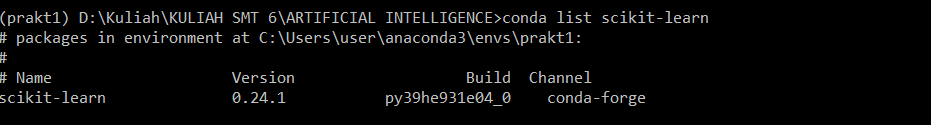
\includegraphics[width=1\textwidth]{figures/1184030/Screenshot (2144).png}
    \caption{Cek Apakah Library Scikit-Learn sudah terinstall}
    \label{fig:my_label}
\end{figure}
    \item Mencoba Loading an example dataset, menjelaskan maksud dari tulisan tersebut dan mengartikan per baris.\\
Loading an example dataset (memuat contoh kumpulan data) maksudnya yaitu scikit-learn memugkinkan kita untuk mengambil atau memuat data standar, misalnya kita mengambil atau memuat data set iris dan digits untuk membuat sebuah klasifikasi dan data set diabetes untuk regresi.\\
\begin{figure}[H]
    \centering
    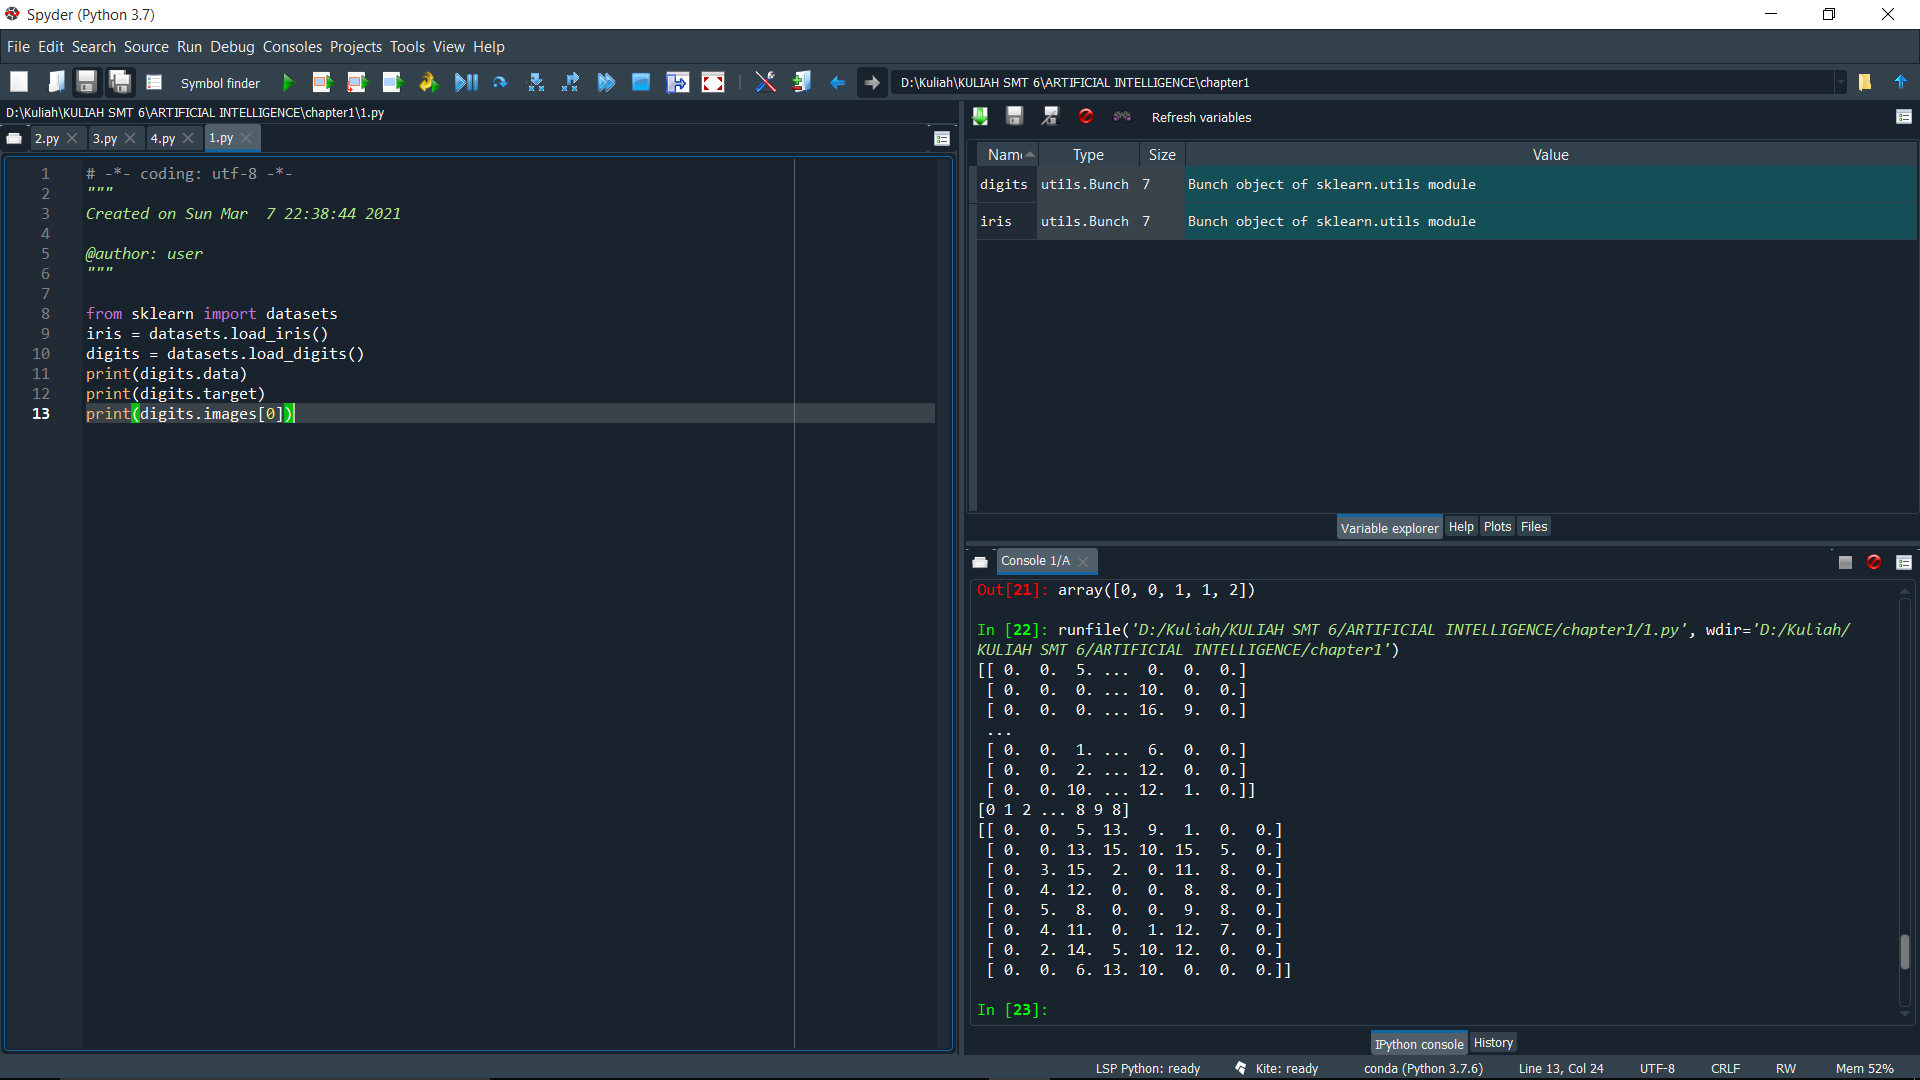
\includegraphics[width=1\textwidth]{figures/1184030/Screenshot (2159).png}
    \caption{Loading an example}
    \label{fig:my_label}
\end{figure}
\begin{lstlisting}
from sklearn import datasets
iris = datasets.load_iris()
digits = datasets.load_digits()
#print(digits.data)
#print(digits.target)
print(digits.images[0])
\end{lstlisting}
Berikut ini penjelasan perbarisnya :\\
\begin{itemize}
    \item from sklearn import datasets\\
    mengimportkan dataset dari library sklearn
    \item iris = datasets.load\_iris()\\
    mendefinisikan variable iris dengan menggunakan load\_iris() dari dataset yang telah diimport sebelumnya
    \item digits = datasets.load\_digits()\\
     mendefinisikan variable digits dengan menggunakan load\_digits() dari dataset yang telah diimport sebelumnya
    \item print(digits.data)\\
    mencetak isi dari variable digits
    \item print(digits.target)\\
    mencetak array target yang sesuai dari variable digits
    \item print(digits.images[0])
\end{itemize}
\item 
Mencoba Learning and predicting, menjelaskan maksud dari tulisan tersebut dan mengartikan per baris.\\

Learning and Predicting (Belajar dan Memprediksi) maksudnya yaitu belajar dari sebuah model dan membuatkan prediksi dalam sebuah gambar. Menggunakan data set digits karena data digits dapat memprediksi, mengingat gambar digit mana yang diwakilinya. \\

\begin{lstlisting}
#learning and predicting
from sklearn import svm
clf = svm.SVC(gamma=0.001, C=100.)
x = clf.fit(digits.data[:-1], digits.target[:-1]) #fit x,y
print(x)
y = clf.predict(digits.data[-1:]) #y = hasil prediksi data baru
print(y)
\end{lstlisting}
berikut ini penjelasan perbarisnya, yaitu :\\
\begin{itemize}
    \item from sklearn import svm\\
    mengimportkan svm pada library sklearn
    \item clf = svm.SVC(gamma=0.001, C=100.)\\
    mendefinisikan variable slf dengan mengambil function SVC dari svm yang telah diimport sebelumnya
    \item x = clf.fit(digits.data[:-1], digits.target[:-1]) \\
    fit x,y
    \item y = clf.predict(digits.data[-1:])\\
mendefinisikan hasil prediksi data baru
\end{itemize}
\item 
mencoba Model persistence, menjelaskan maksud dari tulisan tersebut dan mengartikan per baris.\\
Model Presistence maksudnya mempertahankan sebuah model agar bisa digunakan di masa depan tanpa perlu melatih kembali atau membuat model itu kembali. Menyimpan model dengan menggunakan pickle atau joblib
\begin{lstlisting}
from sklearn import svm
from sklearn import datasets
clf = svm.SVC()
X, y = datasets.load_iris(return_X_y=True)
clf.fit(X, y)
#contoh menggunakan pickle
import pickle
a = pickle.dumps(clf)
clf2 = pickle.loads(a)
clf2.predict(X[0:1])
y[0]
\end{lstlisting}
\item 
Mencoba Conventions, menjelaskan maksud dari tulisan tersebut dan mengartikan per baris.\\

Conventions (konvensi) maksudnya dapat memprediksi dengan lebih prediktif.\\
\begin{itemize}
    \item Type casting
    \begin{lstlisting}
#conventions type casting
import numpy
from sklearn import random_projection
rng = numpy.random.RandomState(0)
X = rng.rand(10, 2000)
X =numpy.array(X, dtype='float32')
X.dtype #type floatnya 32
transformer = random_projection.GaussianRandomProjection()
X_new = transformer.fit_transform(X)
X_new.dtype #type floatnya 64 
    \end{lstlisting}
    \item Refitting and updating parameters
\begin{lstlisting}
#conventions refitting and updating parameters
import numpy as np #mengimportkan library numpy dan dialiaskan dengan np
from sklearn.datasets import load_iris #mengimportkan load_iris dari sklearn.datasets
from sklearn.svm import SVC #mengimportkan SVC dari sklearn.svm
X, y = load_iris(return_X_y=True)
clf = SVC()
clf.set_params(kernel='linear').fit(X, y)
clf.predict(X[:5])
clf.set_params(kernel='rbf').fit(X, y)
clf.predict(X[:5])
\end{lstlisting}
    \item multiclass vs multilabel fitting
\begin{lstlisting}
#multiclass
from sklearn.svm import SVC
from sklearn.multiclass import OneVsRestClassifier
from sklearn.preprocessing import LabelBinarizer
X = [[1, 2], [2, 4], [4, 5], [3, 2], [3, 1]]
y = [0, 0, 1, 1, 2]
classif = OneVsRestClassifier(estimator=SVC(random_state=0))
classif.fit(X, y).predict(X) #menghasilkan array 1 dimensi

#multiple labels

y = LabelBinarizer().fit_transform(y)
classif.fit(X, y).predict(X) #menghasilkan array 2 dimensi namun, hasil pada array ke 3 dan 4 bernilai 0

#pengklasifikasian array 2 dimensi dengan multilabel yang diprediksi pada tiap instance
from sklearn.preprocessing import MultiLabelBinarizer
y = [[0, 1], [0, 2], [1, 3], [0, 2, 3], [2, 4]]
y = MultiLabelBinarizer().fit_transform(y)
classif.fit(X, y).predict(X)
\end{lstlisting}
\end{itemize}
\end{enumerate}
\section{Penanganan Error}
\begin{enumerate}
	\item
	skrinsut error[hari ke 2](10)
	\item
Tuliskan kode eror dan jenis errornya [hari ke 2](10)
	\item
Solusi pemecahan masalah error tersebut[hari ke 2](10)

\end{enumerate}
%\chapter{Membangun Model Prediksi}

\section{Teori}
Praktek teori penunjang yang dikerjakan(nilai 5 per nomor, untuk hari pertama) :
\begin{enumerate}
\item
binary classificarion ialah suatu bentuk klasifikasi supervised learning dengan berdasarkan label class, dimana pada binary classification, terdapat satu atribut class yang berisikan 2 value. Value tersebut dapat dipresentasikan sebagai nilai positif/negatif, lulus/tidak, true/false, 0/1, spam/tidak, dan sebagainya. hal ini disebut juga sebagai binary classifier.
\par tujuan digunakannya binary classification ialah untuk dapat mencari batas data secara optimal berdasarkan kelas yang ditentukan. biasanya, binary classifier ini digunakan sebagai label suatu tabel, namun tidak menutup kemungkinan bahwa dalam suatu tabel terdapat lebih dari 1 binary classifier, karena dengan penggunaan binary classifier ini dapat memudahkan dalam menentukan label dari suatu tabel.
\par contoh implementasi binary classification yaitu di antaranya :
\begin{enumerate}
    \item ketika hendak mengklasifikasikan email, apakah email tersebut termasuk ke dalam spam atau tidak spam
    \item ketika hendak mengklasifikasikan mahasiswa, apakah lulus atau tidak lulus, berdasar atribut tabel yang lainnya
\end{enumerate}
\item
Jelaskan apa itu supervised learning dan unsupervised learning dan clustering dengan ilustrasi gambar sendiri.
\par supervised learning
Supervised learning merupakan suatu algoritma yang digunakan untuk menen-
tukan suatu prediksi dan klasifikasi berdasarkan variabel x dan variabel y telah
diketahui. Algoritma ini seolah-olah sudah dilatih sehingga dapat menghasilkan
suatu bentuk prediksi dan klasifikasi. Supervised learning menggunakan label di setiap datanya, data yang diklasifikasi dapat berupa klasifikasi (contoh : "lulus", "tidak lulus") ataupun regresi (periode kuliah, nilai).
Algoritma yang dapat digunakan pada supervised learning di antaranya yaitu :
\begin{enumerate}
    \item Classification and Regression
    \item Logistic Regression
    \item Time Series
    \item Model Ensemble
\end{enumerate}
salah satu contohnya, ketika dimiliki data klasifikasi hewan, dengan fitur bentuk gigi, bentuk kuku, ketahanan suhu dan label jenis dengan value karnivora, herbivora, dan omnivora.
dari data tersebut, diklasifikasikan dengan metode classification karena data yang dimiliki ialah data yang bersifat categorical.
\par Unsupervised learning yaitu suatu algoritma penentuan prediksi dimana data
tidak memiliki output/target variablenya (label), sehingga tidak yang mengendalikan
jalannya algoritma suatu program. Berbeda dengan supervised learning, algo-
ritma ini tidak perlu dilatih dahulu untuk dapat mengjasilkan prediksi maupun
klasifikasi.
cara kerja algoritma unsupervised ini dilakukan dengan menggunakan perhitungan kesamaan dari atribut yang dimiliki, ketika setiap atribut dan sifatnya diekstrak dan memiliki kemiripan atau kemiripan terdekat, maka akan dikelompokkan menjadi 1 kelompok (cluster).\\
Algoritma yang dapat digunakan pada metode ini di antaranya yaitu :
\begin{enumerate}
    \item Clustering
    \item Training Model
    \item Anomaly Detection
    \item Association Discovery
\end{enumerate}
Contohnya yaitu diketahui data gambar hewan, maka dari data gambar tersebut akan diekstrak dalam machine learning, untuk kemudian dilakukan clustering berdasar kemiripan yang dimiliki di setiap data gambar tersebut.
\par Clustering ialah suatu metode yang digunakan untuk pengelompokan data berdasarkan kemiripan data tersebut setelah diekstrak, clustering ini umumnya digunakan untuk metode unsupervised learning. contohnya yaitu K-Means Clustering, KNN.
\item
Evaluasi dan Akurasi\\
\begin{itemize}
    \item Evaluasi\\
    Evaluasi ialah suatu kegiatan/proses yang bertujuan untuk dapat menentukan/membuat keputusan berdasarkan sejauh mana tujuan program telah tercapai.\\
    Menurut Abdul Basir (1996), evaluasi ialah suatu proses pengimpulan data secara deskriptif, informatif dan prediktif yang dilaksanakan dengan sistematis dan bertahap sehingga dapat menentukan kebijaksanaan dalam usaha untuk memperbaiki pendidikan.
    \item Akurasi\\
    Akurasi ialah perbandingan prediksi benar (baik positif atau negatif) terhadap keseluruhan data yang digunakan.
    \par contohnya, seperti pada confusion matriks di bawah ini
    \begin{figure}[H]
    \centering
    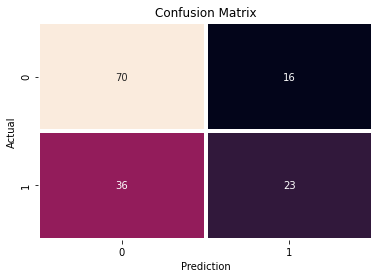
\includegraphics[width=0.5\textwidth]{figures/confusion_matrix.png}
    \caption{Contoh}
    \label{fig:my_label}
    \end{figure}
    dari confusion matrix tersebut, didapatkan
    \begin{itemize}
        \item TP = 70
        \item FP = 16
        \item TN = 36
        \item FN = 23
    \end{itemize}
    yang berarti total data prediksi benar yakni TP + FN = 70 + 23 = 93 data.
    oleh karenanya, akurasi bisa didapatkan dengan
\begin{lstlisting}
Akurasi = (TP + TN ) / (TP+FP+FN+TN) * 100%
Akurasi = 93/145*100%
Akurasi = 64%
\end{lstlisting}
\end{itemize}
\item Confusion Matrix\\
confusion matrix merupakan salah satu model klasifikasi yang digunakan untuk mengukur kinerja suatu model atau klasifikasi.\\
\par confusion matriks memberikan perbandingan hasil klasifikasi yang dihasilkan oleh model, dengan hasil klasifikasi yang sebenarnya dengan bentuk tabel matriks yang berisikan kombinasi nilai prediksi dan nilai aktual seperti berikut :
\begin{figure}[H]
    \centering
    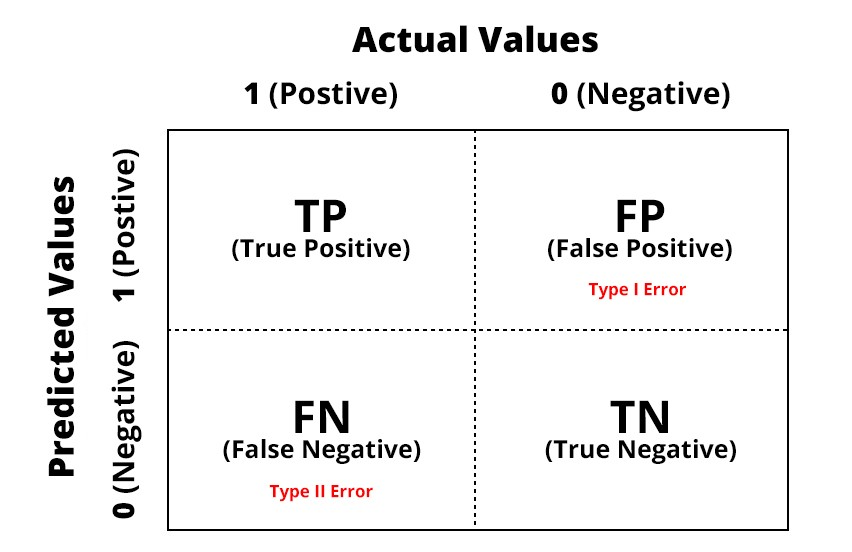
\includegraphics[width=0.50\textwidth]{figures/confusion_matriks.jpeg}
    \caption{Tabel Confusion Matriks}
    \label{fig:my_label}
\end{figure}
\par confusion matrix dibagi menjadi 2, yakni :
\begin{enumerate}
    \item binary classification confusion matrix \\
    ialah confusion matrix yang hanya memiliki 2 value pada label yang digunakan. contohnya ya/tidak, lulus/tidak lulus, baik/buruk, recommend/not recommend.
    \item multiclass classification confusion matrix\\
    ialah confusion matrix yang memiliki multiclass classification pada labelnya, yakni valuenya lebih dari 2. contohnya yaitu sangat buruk/buruk/baik/sangat baik, A/B/C/D/E, sangat tidak recommend/recommend/sangat recommend.
\end{enumerate}
berikut ini kode program untuk membuat visualisasi confusion matrix dengan matplotlib dan seaborn
\begin{lstlisting}
import pandas as pd, seaborn as sns, matplotlib.pyplot as plt, numpy as np
from sklearn.metrics import confusion_matrix
sns.heatmap(confusion_matrix(d_jeruk_test_pass, y_pred),annot=True,linewidths=3,cbar=False)
plt.title('Confusion Matrix')
plt.ylabel('Actual')
plt.xlabel('Prediction')
plt.show()
\end{lstlisting}
berikut ini contoh hasil confusion matrixnya :
\begin{enumerate}
    \item binary
    \begin{figure}[H]
    \centering
    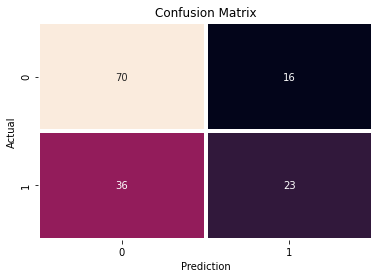
\includegraphics[width=0.75\textwidth]{figures/confusion_matrix.png}
    \caption{Hasil Visualisasi Binary Confusion Matriks}
    \label{fig:my_label}
    \end{figure}
    dari confusion matrix tersebut, didapatkan :
    \begin{itemize}
        \item TP = 70
        \item FP = 16
        \item TN = 36
        \item FN = 23
    \end{itemize}
    \item multiclass
    \begin{figure}[H]
    \centering
    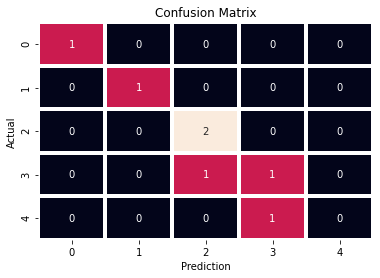
\includegraphics[width=0.75\textwidth]{figures/confusion_matrix2.png}
    \caption{Hasil Visualisasi Multiclass Confusion Matriks}
    \label{fig:my_label}
    \end{figure}
    Dari confusion matriks tersebut, didapat:
    \begin{itemize}
        \item Nilai actual dan nilai predict = 0 berjumlah 1 data
        \item Nilai actual dan nilai predict = 1 berjumlah 1 data
        \item Nilai actual dan nilai predict = 1 berjumlah 1 data
        \item Nilai actual dan nilai predict = 2 berjumlah 2 data
        \item Nilai actual = 3, namun nilai predict = 2 berjumlah 1 data
        \item Nilai actual dan nilai predict = 3, berjumlah 1 data
        \item Nilai actual = 4, namun nilai predict = 3 berjumlah 1 data
    \end{itemize}
Berikut hasil value metrics True Positive, False Positive, True Negative, dan False Negative dari confusion matrix di atas :
\begin{itemize}
    \item Huruf = 0 (A), memiliki representasi :
    \begin{enumerate}
        \item TP0 = 1
        \item FP0 = 0 + 0 + 0 + 0 = 0
        \item TN0 = 1 + 0 + 0 + 0 + 0 +2 + 0 + 0 +0 + 1+ 1 + 0 + 0 +0 + 1 + 0 = 6
        \item FN0  = 0 +0 +0 +0 = 0
    \end{enumerate}
    \item Huruf = 1 ( B), memiliki representasi :
    \begin{enumerate}
        \item TP1 = 1
        \item FP1 = 0 + 0 + 0 + 0 = 0
        \item TN1 = 1 + 0 + 0 + 0 + 0 +2 + 0 + 0 +0 + 1+ 1 + 0 + 0 +0 + 1 + 0 = 6
        \item FN1  = 0 +0 +0 +0 = 0
    \end{enumerate}
    \item Huruf = 2 ( C), memiliki representasi :
    \begin{enumerate}
        \item TP2 = 2
        \item FP2 = 0 + 0 + 0 + 0 = 0
        \item TN2 = 1 + (0*3) + 0 + 1 + (0*2) +(0*2) + 1 + 0 + (0*2) + 1 + 0 = 4
        \item FN2  = 0 +0 +1 +0 = 1
    \end{enumerate}
    \item Huruf = 3 ( D), memiliki representasi :
    \begin{enumerate}
        \item TP3 = 1
        \item FP3 = 0 + 0 + 1 + 0 = 1
        \item TN3 = 1 + (0*3) + 0 + 1 + (0*2) +(0*2) + 2 + (0*2) + (0*4) = 4
        \item FN3  = 0 +0 + 0 + 1 = 1
    \end{enumerate}
    \item Huruf = 4 ( huruf E), memiliki representasi :
    \begin{enumerate}
        \item TP4 = 0
        \item FP4 = 0 + 0 + 0 + 1 = 1
        \item TN4 = 1 + (0*3) + 0 + 1 + (0*2) +(0*2) + 2 + (0*2) + 1 + 1 = 6
        \item FN4  = 0 +0 + 0 + 0 = 0
    \end{enumerate}
\end{itemize}
\end{enumerate}
\item K-fold Cross Validation
Jelaskan bagaimana K-fold cross validation bekerja dengan gambar ilustrasi contoh buatan sendiri.\\
k-fold cross valdation ialah metode tambahan yang digunakan untuk dapat diperoleh hasil akurasi yang lebih maksimal. dinamakan k-fold cross validation karena dilakukan percobaan sebanyak k kali dengan menggunakan model dan parameter yang sama.\\
\par cross validation juga ialah teknik pengukuran vaidasi yang merupakan bentuk pengembangan dari model Split validation, yakni dilakukan dengan mengukur training error dengan melakukan uji menggunakan data testing.
berikut ini fungsi dari digunakannya k-fold cross validation, yakni :\\
\begin{enumerate}
    \item mengukur performa suatu model dengan melalui percobaan sebanyak k kali
    \item meningkatkan tingkat performansi model tersebut
    \item mengolah dataset dengan menggunakan kelas yang seimbang
    \item pengambilan sampel test yang lebih terstruktur
    \item menjangkau pengujian yang lebih efisien
\end{enumerate}
berikut ini contoh implementasi k-fold cross validation, seperti pada tabel berikut :
\begin{figure}[H]
    \centering
    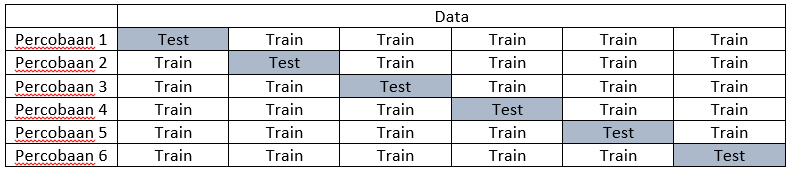
\includegraphics[width=0.75\textwidth]{figures/k-fold.png}
    \caption{contoh K-fold cross validation}
    \label{fig:my_label}
\end{figure}
dari contoh gambar di atas, dapat dibaca seperti berikut :
\begin{itemize}
    \item pada percobaan 1, data 1 digunakan untuk data testing, sisanya digunakan sebagai data training
    \item pada percobaan 2, data 2 digunakan untuk data testing, sisanya digunakan sebagai data training
    \item pada percobaan 3, data 3 digunakan untuk data testing, sisanya digunakan sebagai data training
    \item pada percobaan 4, data 4 digunakan untuk data testing, sisanya digunakan sebagai data training
    \item pada percobaan 5, data 5 digunakan untuk data testing, sisanya digunakan sebagai data training
    \item pada percobaan 6, data 6 digunakan untuk data testing, sisanya digunakan sebagai data training
\end{itemize}
sehingga, dapat disimpulkan bahwa, pada setiap percobaan testing validation selama k kali, data testing yang digunakan berbeda, begitu pula dengan data trainnya, sehingga memungkinkan agar semua data dapat dilakukan uji validasi supaya memaksimalkan akurasi dari model yang digunakan.
\item
Jelaskan apa itu decision tree dengan gambar ilustrasi contoh buatan sendiri.\\
Desicion tree ialah suatu model klasifikasi yang digunakan untuk melakukan pengambilan keputusan dengan menggunakan struktur pohon/hierarki.
metode ini menggabungkan 2 jenis pohon, yakni
\begin{enumerate}
    \item Classification tree
    \item Regression tree
\end{enumerate}
berikut ini contoh decision tree
\begin{figure}[H]
    \centering
    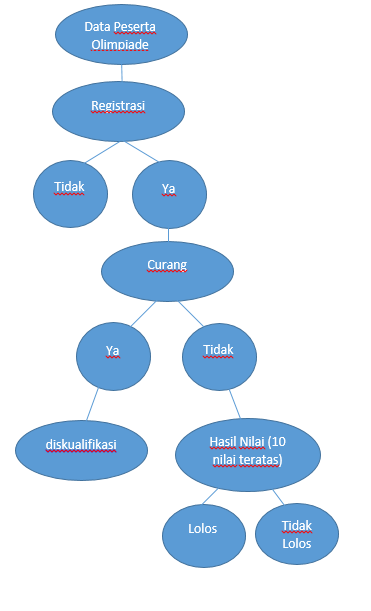
\includegraphics[width=0.75\textwidth]{figures/decisiontree.png}
    \caption{contoh decision dengan classification tree}
    \label{fig:my_label}
\end{figure}
\item Information Gain dan Entropy\\
\begin{enumerate}
    \item Information Gain\\
    Information Gain ialah salah satu metode yang digunakan untuk seleksi fitur, yakni mengukur efektifitas dari atribut yang digunakan dalam melakukan pengklasifikasian data.
    \item Entropy\\
    Entropy ialah suatu nilai yang berisikan informasi ukuran ketidakpastian (impurity) atribut dalam kumpulan objek data dalam satuan bit. semakin sedikit value dari atribut label, maka makin kecil pula nilai entropy yang dihasilkan. Sebaliknya, apabila nilai label multiclass, maka semakin besar pula nilai entropy yang dihasilkan.\\
    Contohnya, ketika dataset A dengan label yang bernilai positif dan negatif, dibandingkan dengan dataset B yang memiliki label tidak direkomensasi, direkomendasikan, dan sangat direkomendasikan. Maka, dari contoh tersebut, entropy dari dataset A lebih kecil dibandingkan dengan dataset B.
\begin{figure}[H]
    \centering
    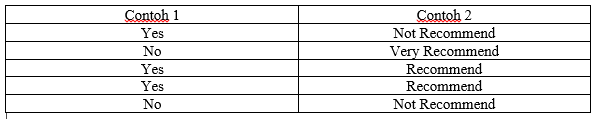
\includegraphics[width=0.75\textwidth]{figures/example.png}
    \caption{contoh atribut}
    \label{fig:my_label}
\end{figure}
dengan contoh tabel di atas, atribut contoh 1 akan memiliki nilai entropy yang lebih kecil dibandingkan dengan atribut contoh 2.
\end{enumerate}
\end{enumerate}

\section{ Praktikum Scikit-learn}
Dataset ambil di https://github.com/PacktPublishing/Python-Artificial-Intelligence-Projects-for-Beginners folder Chapter01.
Tugas anda adalah, dataset ganti menggunakan \textbf{student-mat.csv} dan mengganti semua nama variabel dari kode di bawah ini dengan nama-nama makanan (NPM mod 3=0), kota (NPM mod 3=1), buah (NPM mod 3=2), . Jalankan satu per satu kode tersebut di spyder dengan menggunakan textit{Run current cell}. Kemudian Jelaskan dengan menggunakan bahasa yang mudah dimengerti dan bebas plagiat dan wajib skrinsut dari komputer sendiri masing masing nomor di bawah ini(nilai 5 masing masing pada hari kedua).

\begin{enumerate}
\item
\begin{lstlisting}
# NPM = 1184030
# NPM%3
# import library pandas
import pandas as pd
# load dataset student-mat.csv
d_apel = pd.read_csv('student-mat.csv', sep=';')
# menghitung length dataset csv
len(d_apel)
# generate binary label (pass/fail) berdasar nilai G1+G2+G3, apabila total >= 35, maka bernilai 1, jika tidak maka 0
d_apel['pass'] = d_apel.apply(lambda row: 1 if (row['G1']+row['G2']+row['G3']) 
										>= 35 else 0, axis=1)
# drop row G1, G2 dan G3
d_apel = d_apel.drop(['G1', 'G2', 'G3'], axis=1)
# menampilkan 5 data teratas
d_apel.head()
# use one-hot encoding on categorical columns
d_apel = pd.get_dummies(d_apel, columns=['sex', 'school', 'address', 
								'famsize',
								'Pstatus', 'Mjob', 'Fjob', 'reason', 'guardian', 'schoolsup', 
								'famsup', 'paid', 'activities','nursery', 'higher', 'internet',
								'romantic'])
# menampilkan 5 data teratas
d_apel.head()
# shuffle rows
d_jeruk = d_apel.sample(frac=1)
# split training and testing data
d_jeruk_train = d_jeruk[:250]
d_jeruk_test = d_jeruk[250:]
# train atribut drop row pass
d_jeruk_train_att = d_jeruk_train.drop(['pass'], axis=1)
# train label menggunakan row pass
d_jeruk_train_pass = d_jeruk_train['pass']
# test atribut drop row pass
d_jeruk_test_att = d_jeruk_test.drop(['pass'], axis=1)
# test label menggunakan row pass
d_jeruk_test_pass = d_jeruk_test['pass']
# atribut drop row pass
d_jeruk_att = d_jeruk.drop(['pass'], axis=1)
# menggunakan row pass untuk label
d_jeruk_pass = d_jeruk['pass']

# import library
import numpy as np
# print number of passing students in whole dataset:
print("Passing: %d out of %d (%.2f%%)" % (np.sum(d_jeruk_pass), len(d_jeruk_pass), 
	       100*float(np.sum(d_jeruk_pass)) / len(d_jeruk_pass)))

# import library
from sklearn import tree
# instansiasi desicion tree classifier
melon = tree.DecisionTreeClassifier(criterion="entropy", max_depth=5)
# fit decision tree
melon = melon.fit(d_jeruk_train_att, d_jeruk_train_pass)
# import library graphviz untuk visualisasi
import graphviz
# instansiasi graphviz dari fit decision tree sebelumnya
mangga = tree.export_graphviz(melon, out_file=None, label="all", 
									impurity=False, proportion=True,
	                                feature_names=list(d_jeruk_train_att), 
									class_names=["fail", "pass"], 
	                                filled=True, rounded=True)
# buat variabel grafik visualisasi tree
graph = graphviz.Source(mangga)
# jalankan visualisasinya
graph
\end{lstlisting}
\item
\begin{lstlisting}
# save tree
tree.export_graphviz(melon, out_file="student-performance.dot", 
						 label="all", impurity=False, 
						 proportion=True,
	                     feature_names=list(d_train_att), 
	                     class_names=["fail", "pass"], 
	                     filled=True, rounded=True)
\end{lstlisting}
\item
\begin{lstlisting}
# cek score
melon.score(d_jeruk_test_att, d_jeruk_test_pass)
\end{lstlisting}
\item
\begin{lstlisting}
# import cross val score untuk cek cross validation score
from sklearn.model_selection import cross_val_score
# cek cross validation score
nangka_score = cross_val_score(melon, d_jeruk_att, d_jeruk_pass, cv=5)
# show average score and +/- two standard deviations away 
#(covering 95% of scores)
# print akurasi
print("Accuracy: %0.2f (+/- %0.2f)" % (nangka_score.mean(), nangka_score.std() * 2))
\end{lstlisting}
\item 
\begin{lstlisting}
# buat akurasi max depth
for max_depth in range(1, 20):
	    melon = tree.DecisionTreeClassifier(criterion="entropy", 
			max_depth=max_depth)
	    nangka_score = cross_val_score(melon, d_jeruk_att, d_jeruk_pass, cv=5)
	    print("Max depth: %d, Accuracy: %0.2f (+/- %0.2f)" % 
				(max_depth, nangka_score.mean(), nangka_score.std() * 2)
			 )
\end{lstlisting}
\item
\begin{lstlisting}
# buat akurasi depth acc
depth_acc = np.empty((19,3), float)
i = 0
for max_depth in range(1, 20):
    melon = tree.DecisionTreeClassifier(criterion="entropy", 
		max_depth=max_depth)
    nangka_score = cross_val_score(melon, d_jeruk_att, d_jeruk_pass, cv=5)
    depth_acc[i,0] = max_depth
    depth_acc[i,1] = nangka_score.mean()
    depth_acc[i,2] = nangka_score.std() * 2
    i += 1
# jalankan dept_acc
depth_acc
\end{lstlisting}
\item 
\begin{lstlisting}
	import matplotlib.pyplot as plt
	fig, ax = plt.subplots()
	ax.errorbar(depth_acc[:,0], depth_acc[:,1], yerr=depth_acc[:,2])
	plt.show()
\end{lstlisting}
\end{enumerate}


\section{Penanganan Error}
Dari percobaan yang dilakukan di atas, error yang kita dapatkan di dokumentasikan dan di selesaikan(nilai 5 hari kedua):
\begin{enumerate}
	\item Screenshoot Error
\begin{figure}[H]
    \centering
    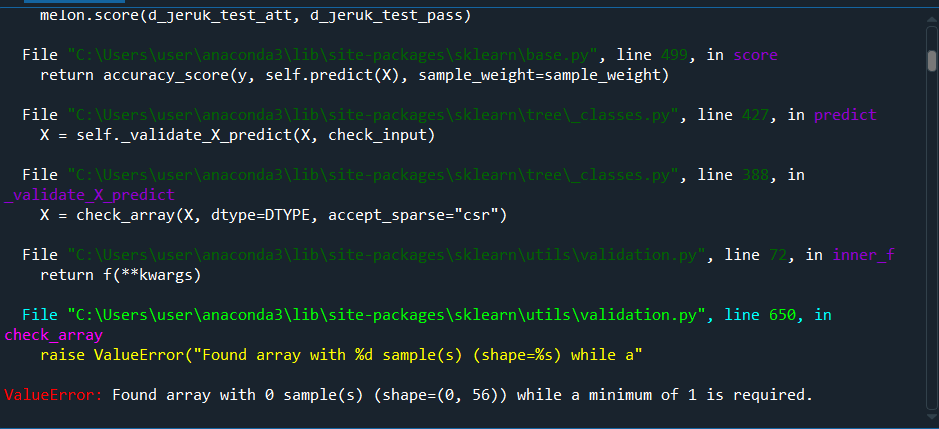
\includegraphics[width=1\textwidth]{figures/Screenshot (2341).png}
    \caption{Error}
    \label{fig:my_label}
\end{figure}
	\item
Kode eror dan jenis errornya\\
\begin{lstlisting}
ValueError: Found array with 0 sample(s) (shape=(0, 56)) while a minimum of 1 is required.
\end{lstlisting}
	\item Solusi pemecahan masalah error\\
solusi yang dilakukan ialah dengan melakukan pengecekan kembali terhadap data yang ditest dan ditrain, di source code yang sebelumnya, digunakan 500 data awal pada data train, dan setelah 500 data awal di data test, namun pada praktikum kali ini, data yang digunakan bahkan tidak lebih dari 500, melainkan hanya 395. sehingga memunculkan error tersebut.
sehingga solusinya yakni mengubah banyak data yang displit untuk data train dan data test dengan menyesuaikan jumlah datanya, disini saya mengubah menjadi 250 data awal untuk data training, dan sisanya untuk data testingnya
\end{enumerate}
%\chapter{Prediksi dengan Random Forest}

Untuk pratikum saati ini menggunakan buku \textit{Python Artificial Intelligence Projects for Beginners}\cite{eckroth2018python}. Dengan praktek menggunakan python 3 dan editor anaconda dan library python scikit-learn.
Kode program ada di https://github.com/PacktPublishing/Python-Artificial-Intelligence-Projects-for-Beginners .
Tujuan pembelajaran pada pertemuan pertama antara lain:
\begin{enumerate}
\item
Mengerti implementasi klasifikasi dan teknik evaluasi
\item
Memprediksi spesies burung dengan random forest
\item
Memahami Confusion Matrix.
\end{enumerate}
Tugas dengan cara dikumpulkan dengan pull request ke github dengan menggunakan latex pada repo yang dibuat oleh asisten riset. Kode program menggunakan input listing ditaruh di folder src ekstensi .py dan dipanggil ke latex dengan input listings. Tulisan dan kode tidak boleh plagiat, menggunakan bahasa indonesia yang sesuai dengan gaya bahasa buku teks.

\section{Teori}
Random Forest adalah hasil voting dari beberapa decission tree yang masing-masing memegang atribut yang berbeda. Jadi setiap decission tree spesifik terhadap atribut tersebut yang merupakan bagian kecil dari keseluruhan atribut di data set. Hindari RF jika atribut terlalu sedikit untuk membentuk beberapa tree. Pada praktek kali ini mengggunakan dataset spesies burung yang diambil dari situs 
(http://www.vision.caltech.edu/visipedia/CUB-200-2011.html). Didalamnya terdapat 12.000 foto dari 200 spesies yang berbeda. Yang akan kita pakai untuk RF hanya atribut dari burunynya saja seperti ukuran, bentuk dan warna. Data tersebut diberi label secara manual oleh manusia dengan memanfaatkan jasa dari Amazon's Mechanical Turk.

\subsection{Random Forest}
Pertama dataset kita baca terlebih dahulu.
\begin{lstlisting}[caption=Membaca data file txt,label={lst:fungsisederhana}]
import pandas as pd

# some lines have too many fields (?), so skip bad lines
imgatt = pd.read_csv("data/CUB_200_2011/attributes/image_attribute_labels.txt",
                     sep='\s+', header=None, error_bad_lines=False, warn_bad_lines=False,
                     usecols=[0,1,2], names=['imgid', 'attid', 'present'])

\end{lstlisting}

Melihat sebagian data awal, dengan menggunakan listing \ref{lst:3.1}.

\begin{lstlisting}[caption=Melihat sebagian data awal,label={lst:3.1}]
imgatt.head()
\end{lstlisting}

Melihat jumlah data menggunakan listing \ref{lst:3.2}.
\begin{lstlisting}[caption=Mengetahui jumlah data,label={lst:3.2}]
imgatt.shape
\end{lstlisting}

Merubah atribut menjadi kolom dengan menggunakan pivot layaknya excel. lalu kita cek isinya dengan menggunakan perintah pada listing \ref{lst:3.3}.
\begin{lstlisting}[caption=Pivot dataset,label={lst:3.3}]
imgatt2 = imgatt.pivot(index='imgid', columns='attid', values='present')

imgatt2.head()
imgatt2.shape
\end{lstlisting}


Sekarang kita akan meload jawabannya yang berisi apakah burung itu termasuk dalam spesies yang mana. Dua kolomnya adalah imgid dan label. Dan melakukan pivot yang mana imgid menjadi index yang artinya unik perintahnya ada di listing \ref{lst:3.6}. Lalu kita cek kembali datanya. 
\begin{lstlisting}[caption=membaca dataset label file txt,label={lst:3.6}]
imglabels = pd.read_csv("data/CUB_200_2011/image_class_labels.txt", 
                        sep=' ', header=None, names=['imgid', 'label'])

imglabels = imglabels.set_index('imgid')


imglabels.head()
imglabels.shape
\end{lstlisting}

Karena isinya sama kita bisa melakukan join antara dua data. Sehingga kita akan mendapatkan data ciri dan data jawabannya atau labelnya sehingga bisa dikatekorikan supervised learning. maka perintah untuk menggabungkan kedua data dan kemudian kita melakukan pemisahan antara data set untuk training dan test dengan perintah di listing \ref{lst:3.7}.
\begin{lstlisting}[caption=Menggabungkan field dari dua file terpisah,label={lst:3.7}]
df = imgatt2.join(imglabels)
df = df.sample(frac=1)
\end{lstlisting}

Kemudian drop label yang didepan, dan gunakan label yang paling belakang yang baru di join dengan perintah listing \ref{lst:3.8}.
\begin{lstlisting}[caption=Memisahkan dan memilih label,label={lst:3.8}]
df_att = df.iloc[:, :312]
df_label = df.iloc[:, 312:]
\end{lstlisting}
Kita bisa mengecek isinya dengan perintah listing \ref{lst:3.9}.
\begin{lstlisting}[caption=Melihat isi masing masing data frame,label={lst:3.9}]
df_att.head()
df_label.head()
\end{lstlisting}

Kita bagi menjadi dua bagian, 8000 row pertama sebagai data training sisanya sebagai data testing dengan perintah listing \ref{lst:3.10}.
\begin{lstlisting}[caption=Pembagian data training dan test,label={lst:3.10}]
df_train_att = df_att[:8000]
df_train_label = df_label[:8000]
df_test_att = df_att[8000:]
df_test_label = df_label[8000:]

df_train_label = df_train_label['label']
df_test_label = df_test_label['label']
\end{lstlisting}

Kita panggil kelas RandomForestClassifier. max features diartikan sebagai berapa banyak kolom pada setiap tree dengan perintah listing \ref{lst:3.11}.
\begin{lstlisting}[caption=Instansiasi kelas Random Forest,label={lst:3.11}]
from sklearn.ensemble import RandomForestClassifier
clf = RandomForestClassifier(max_features=50, random_state=0, n_estimators=100)

\end{lstlisting}
Kemudian lakukan fit untuk membangun random forest yang sudah ditentukan dengan maksimum fitur sebanya 50 untuk perpohonnya dengan perintah listing \ref{lst:3.12}.

\begin{lstlisting}[caption=Fitting random forest dengan dataset training,label={lst:3.12}]
clf.fit(df_train_att, df_train_label)
\end{lstlisting}
Hasilnya bisa kita dapatkan dengan perintah predict dengan perintah listing \ref{lst:3.13}.
\begin{lstlisting}[caption=Melihat Hasil prediksi,label={lst:3.13}]
print(clf.predict(df_train_att.head()))
\end{lstlisting}

Untuk besaran akurasinya dengan perintah listing \ref{lst:3.14}
\begin{lstlisting}[caption=Score perolehan dari klasifikasi,label={lst:3.14}]
clf.score(df_test_att, df_test_label)
\end{lstlisting}

\subsection{Confusion Matrix}
Dari RF kita coba petakan ke dalam Confusion Matrix dan lihat hasilnya dengan perintah listing \ref{lst:3.15}.
\begin{lstlisting}[caption=Membuat Confusion Matrix,label={lst:3.15}]
from sklearn.metrics import confusion_matrix
pred_labels = clf.predict(df_test_att)
cm = confusion_matrix(df_test_label, pred_labels)

cm
\end{lstlisting}

Kemudian kita plot dengan perintah
\begin{lstlisting}[caption=Plotting Confusion Matrix,label={lst:3.16}]
import matplotlib.pyplot as plt
import itertools
def plot_confusion_matrix(cm, classes,
                          normalize=False,
                          title='Confusion matrix',
                          cmap=plt.cm.Blues):
    """
    This function prints and plots the confusion matrix.
    Normalization can be applied by setting `normalize=True`.
    """
    if normalize:
        cm = cm.astype('float') / cm.sum(axis=1)[:, np.newaxis]
        print("Normalized confusion matrix")
    else:
        print('Confusion matrix, without normalization')

    print(cm)

    plt.imshow(cm, interpolation='nearest', cmap=cmap)
    plt.title(title)
    #plt.colorbar()
    tick_marks = np.arange(len(classes))
    plt.xticks(tick_marks, classes, rotation=90)
    plt.yticks(tick_marks, classes)

    fmt = '.2f' if normalize else 'd'
    thresh = cm.max() / 2.
    #for i, j in itertools.product(range(cm.shape[0]), range(cm.shape[1])):
    #    plt.text(j, i, format(cm[i, j], fmt),
    #             horizontalalignment="center",
    #             color="white" if cm[i, j] > thresh else "black")

    plt.tight_layout()
    plt.ylabel('True label')
    plt.xlabel('Predicted label')

\end{lstlisting}

 Agar plot sumbunya sesuai dengan nama datanya maka kita set dengan perintah
\begin{lstlisting}[caption=Membaca file classes.txt,label={lst:3.17}]
birds = pd.read_csv("data/CUB_200_2011/classes.txt",
                    sep='\s+', header=None, usecols=[1], names=['birdname'])
birds = birds['birdname']
birds

\end{lstlisting}

Lalu kita plot
\begin{lstlisting}[caption=Plot hasil perubahan label,label={lst:3.18}]
import numpy as np
np.set_printoptions(precision=2)
plt.figure(figsize=(60,60), dpi=300)
plot_confusion_matrix(cm, classes=birds, normalize=True)
plt.show()
\end{lstlisting}



\subsection{Mencoba dengan metode Decission Tree dan SVM}
Kita coba menggunakan Decission tree 
\begin{lstlisting}[caption=Mencoba klasifikasi dengan decission tree dengan dataset yang sama,label={lst:3.19}]
from sklearn import tree
clftree = tree.DecisionTreeClassifier()
clftree.fit(df_train_att, df_train_label)
clftree.score(df_test_att, df_test_label)
\end{lstlisting}
Kita coba menggunakan SVM
\begin{lstlisting}[caption=Mencoba klasifikasi dengan SVM dengan dataset yang sama,label={lst:3.20}]
from sklearn import svm
clfsvm = svm.SVC()
clfsvm.fit(df_train_att, df_train_label)
clfsvm.score(df_test_att, df_test_label)
\end{lstlisting}

\subsection{Pengecekan Cross Validation}
Pengeceken Cross Validation untuk random forest
\begin{lstlisting}[caption=Hasil Cross Validation random forest,label={lst:3.21}]
from sklearn.model_selection import cross_val_score
scores = cross_val_score(clf, df_train_att, df_train_label, cv=5)
# show average score and +/- two standard deviations away (covering 95% of scores)
print("Accuracy: %0.2f (+/- %0.2f)" % (scores.mean(), scores.std() * 2))
\end{lstlisting}
untuk decission tree
\begin{lstlisting}[caption=Hasil Cross Validation Decission Tree,label={lst:3.22}]
scorestree = cross_val_score(clftree, df_train_att, df_train_label, cv=5)
print("Accuracy: %0.2f (+/- %0.2f)" % (scorestree.mean(), scorestree.std() * 2))
\end{lstlisting}
untuk SVM
\begin{lstlisting}[caption=Hasil Cross Validation SVM,label={lst:3.23}]
scoressvm = cross_val_score(clfsvm, df_train_att, df_train_label, cv=5)
print("Accuracy: %0.2f (+/- %0.2f)" % (scoressvm.mean(), scoressvm.std() * 2))
\end{lstlisting}



\subsection{Pengamatan komponen informasi}
Untuk mengetahui berapa banyak tree yang dibuat, berapa banyak atribut yang dipakai dan informasi lainnya menggunakan kode
\begin{lstlisting}[caption=Melakukan Pengamatan komponen informasi,label={lst:3.24}]
max_features_opts = range(5, 50, 5)
n_estimators_opts = range(10, 200, 20)
rf_params = np.empty((len(max_features_opts)*len(n_estimators_opts),4), float)
i = 0
for max_features in max_features_opts:
    for n_estimators in n_estimators_opts:
        clf = RandomForestClassifier(max_features=max_features, n_estimators=n_estimators)
        scores = cross_val_score(clf, df_train_att, df_train_label, cv=5)
        rf_params[i,0] = max_features
        rf_params[i,1] = n_estimators
        rf_params[i,2] = scores.mean()
        rf_params[i,3] = scores.std() * 2
        i += 1
        print("Max features: %d, num estimators: %d, accuracy: %0.2f (+/- %0.2f)" %               (max_features, n_estimators, scores.mean(), scores.std() * 2))

\end{lstlisting}
Dan kita bisa melakukan plot informasi ini dengan kode
\begin{lstlisting}[caption=Plot Komponen informasi agar bisa dibaca,label={lst:3.25}]
import matplotlib.pyplot as plt
from mpl_toolkits.mplot3d import Axes3D
from matplotlib import cm
fig = plt.figure()
fig.clf()
ax = fig.gca(projection='3d')
x = rf_params[:,0]
y = rf_params[:,1]
z = rf_params[:,2]
ax.scatter(x, y, z)
ax.set_zlim(0.2, 0.5)
ax.set_xlabel('Max features')
ax.set_ylabel('Num estimators')
ax.set_zlabel('Avg accuracy')
plt.show()
\end{lstlisting}




\section{Soal Teori}
Praktek teori penunjang yang dikerjakan(nilai 5 per nomor, untuk hari pertama) :
\begin{enumerate}
\item
Jelaskan apa itu random forest, sertakan gambar ilustrasi buatan sendiri.
\item
Jelaskan cara membaca dataset kasus dan artikan makna setiap file dan isi field masing masing file.
\item
Jelaskan apa itu cross validation
\item
Jelaskan apa arti score 44\% pada random forest, 27\% pada decission tree dan 29\%dari SVM.
\item
Jelaskan bagaimana cara membaca confusion matriks dan contohnya memakai gambar atau ilustrasi sendiri.
\item
Jelaskan apa itu voting pada random forest disertai dengan ilustrasi gambar sendiri.
\end{enumerate}

\section{Praktek Program}
Tugas anda adalah,praktekkan dan jelaskan dengan menggunakan bahasa yang mudah dimengerti dan bebas plagiat dan wajib skrinsut dari komputer sendiri masing masing nomor di bawah ini(nilai 5 masing masing pada hari kedua).

\begin{enumerate}
\item buat aplikasi sederhana menggunakan pandas dan jelaskan arti setiap baris kode yang dibuat(harus beda dengan teman sekelas)
\item buat aplikasi sederhana menggunakan numpy dan jelaskan arti dari setiap baris kode yang dibuat(harus beda dengan teman sekelas)
\item buat aplikasi sederhana menggunakan matplotlib dan jelaskan arti dari setiap baris kode(harus beda dengan teman sekelas)
\item jalankan program klasifikasi Random Fores pada bagian teori bab ini. Tunjukkan keluarannya dari komputer sendiri dan artikan maksud setiap luaran yang didapatkan.
\item jalankan program confusion matrix pada bagian teori bab ini. Tunjukkan keluarannya dari komputer sendiri dan artikan maksud setiap luaran yang didapatkan.
\item jalankan program klasifikasi SVM dan Decission Tree pada bagian teori bab ini. Tunjukkan keluarannya dari komputer sendiri dan artikan maksud setiap luaran yang didapatkan.
\item jalankan program cross validaiton pada bagian teori bab ini. Tunjukkan keluarannya dari komputer sendiri dan artikan maksud setiap luaran yang didapatkan.
\item jalankan program pengamatan komponen informasi pada bagian teori bab ini. Tunjukkan keluarannya dari komputer sendiri dan artikan maksud setiap luaran yang didapatkan.
\end{enumerate}


\section{Penanganan Error}
Dari percobaan yang dilakukan di atas, error yang kita dapatkan di dokumentasikan dan di selesaikan(nilai 5 per error yang ditangani. Untuk hari kedua):

\begin{enumerate}
	\item skrinsut error
	\item Tuliskan kode eror dan jenis errornya
	\item Solusi pemecahan masalah error tersebut
\end{enumerate}

\section{Presentasi Tugas}
Pada pertemuan ketiga ini, diadakan tiga penilaiain yaitu penilaian untuk tugas mingguan seperti sebelumnya dengan nilai maksimal 100. Kemudian dalam satu minggu kedepan maksimal sebelum waktu mata kuliah kecerdasan buatan. Ada presentasi tugas bab ini dan bab sebelumnya dengan nilai presentasi yang terpisah masing-masing 100. Jadi ada tiga komponen penilaiain pada pertemuan ini yaitu :
\begin{enumerate}
	\item tugas minggu hari ini dan besok (maks 100). pada chapter ini
	\item presentasi decission tree (maks 100). Mempraktekkan kode python dan menjelaskan cara kerjanya.
	\item presentasi Random Forest (maks 100).Mempraktekkan kode python dan menjelaskan cara kerjanya.
\end{enumerate}
Waktu presentasi pada jam kerja di IRC. Kriteria penilaian presentasi sangat sederhana, jika presenter tidak bisa menjawab pertanyaan asisten maka nilai nol. Jika semua pertanyaan bisa dijawab maka nilai 100. Presentasi bisa diulang apabila nilai nol sampai bisa mendapatkan nilai 100 dalam waktu satu minggu kedepan.



%\chapter{Pengelolaan File CSV}

Tujuan pembelajaran pada pertemuan keempat antara lain:
\begin{enumerate}
\item
Mengenal file CSV dan fungsinya 
\item
Mengerti cara memakai library CSV
\item
Mengerti cara memakai library pandas
\item
Mengatasi Error yang terjadi akibat pemakaian library csv dan pandas
\item
Try Except
\end{enumerate}
Tugas dengan cara dikumpulkan dengan pull request ke github dengan menggunakan latex pada repo yang dibuat oleh asisten IRC. Kode program dipisah dalam folder src NPM.py yang berisi praktek dari masing-masing tugas file terpisah sesuai nomor yang kemudian dipanggil menggunakan input listing ke dalam file latex penjelasan atau nomor pengerjaan. Masing masing soal bernilai 5 dengan total nilai 100. Gunakan bahasa yang baku dan bebas plagiat dengan dibuktikan hasil scan plagiarisme. Serta hasil scrinsut dari komputer sendiri, dan kode hasil sendiri. Pengerjaan menggunakan latex dan harus menyertakan file pdf hasil compile pdflatex, jika tidak diskon 50\%.


\section{Pemahaman Teori}
Kerjakan soal berikut ini, masing masing bernilai 5. Untuk hari pertama.
Praktek teori penunjang yang dikerjakan dengan deadline besok jam 4 pagi:
\begin{enumerate}
\item
Apa itu fungsi file csv, jelaskan sejarah dan contoh
\item
Aplikasi-aplikasi apa saja yang bisa menciptakan file csv?
\item
Jelaskan bagaimana cara menulis dan membaca file csv di excel atau spreadsheet
\item
Jelaskan sejarah library csv
\item
Jelaskan sejarah library pandas
\item
Jelaskan fungsi-fungsi yang terdapat di library csv
\item
Jelaskan fungsi-fungsi yang terdapat di library pandas
\end{enumerate}

\section{Ketrampilan Pemrograman}
Kerjakan soal berikut ini, masing masing bernilai 5 untuk hari kedua, lusa jam 4 pagi. Soalnya adalah:

\begin{enumerate}
\item
Buatlah fungsi (file terpisah/library dengan nama NPM\_csv.py) untuk membuka file csv dengan lib csv mode list
\item
Buatlah fungsi (file terpisah/library dengan nama NPM\_csv.py) untuk membuka file csv dengan lib csv mode dictionary
\item
Buatlah fungsi (file terpisah/library dengan nama NPM\_pandas.py) untuk membuka file csv dengan lib pandas mode list
\item
Buatlah fungsi (file terpisah/library dengan nama NPM\_pandas.py) untuk membuka file csv dengan lib pandas mode dictionary
\item
Buat fungsi baru di NPM\_pandas.py untuk mengubah format tanggal menjadi standar dataframe
\item
Buat fungsi baru di NPM\_pandas.py untuk mengubah index kolom
\item
Buat fungsi baru di NPM\_pandas.py untuk mengubah atribut atau nama kolom
\item
Buat program main.py yang menggunakan library NPM\_csv.py yang membuat dan membaca file csv
\item
Buat program main2.py yang menggunakan library NPM\_pandas.py yang membuat dan membaca file csv
\end{enumerate}




\section{Ketrampilan Penanganan Error}
Kerjakan soal berikut ini, masing masing bernilai 5(hari kedua). Bagian Penanganan error dari script python.
\begin{enumerate}
\item
Tuliskan peringatan error yang didapat dari mengerjakan praktek ketiga ini, dan jelaskan cara penanganan error tersebut.
dan Buatlah satu fungsi yang menggunakan gunakan try except untuk menanggulangi error tersebut.
\end{enumerate}



\section{Presentasi Tugas}
Pada pertemuan ini, diadakan dua penilaiain yaitu penilaian untuk tugas mingguan seperti sebelumnya dengan nilai maksimal 100. Kemudian dalam satu minggu kedepan maksimal sebelum waktu mata kuliah kecerdasan buatan. Ada presentasi kematerian dengan nilai presentasi yang terpisah masing-masing 100. Jadi ada tiga komponen penilaiain pada pertemuan ini yaitu :
\begin{enumerate}
	\item tugas minggu hari ini dan besok (maks 100). pada chapter ini
	\item presentasi csv (maks 100). Mempraktekkan kode python dan menjelaskan cara kerjanya.
\end{enumerate}
Waktu presentasi pada jam kerja di IRC. Kriteria penilaian presentasi sangat sederhana, presenter akan ditanyai 20(10 pertanyaan program, 10 pertanyaan teori) pertanyaan tentang pemahamannya menggunakan python untuk kecerdasan buatan. jika presenter tidak bisa menjawab satu pertanyaan asisten maka nilai nol. Jika semua pertanyaan bisa dijawab maka nilai 100. Presentasi bisa diulang apabila gagal, sampai bisa mendapatkan nilai 100 dalam waktu satu minggu kedepan.





%\chapter{Vektorisasi kata dan dokumen}

Untuk pratikum saati ini menggunakan buku \textit{Python Artificial Intelligence Projects for Beginners}\cite{eckroth2018python}. Dengan praktek menggunakan python 3 dan editor anaconda dan library python scikit-learn.
Kode program ada di https://github.com/awangga/Python-Artificial-Intelligence-Projects-for-Beginners .
Tujuan pembelajaran pada pertemuan pertama antara lain:
\begin{enumerate}
\item
Mengerti konsep dasar vektorisasi pada kata dan dokumen
\item
Mengerti teknik machine learning untuk similaritas kata dan dokumen
\item
Memahami score dari berbagai teknik klasifikasi
\end{enumerate}

Tugas dengan cara dikumpulkan dengan pull request ke github dengan menggunakan latex pada repo yang dibuat oleh asisten riset. Kode program menggunakan input listing ditaruh di folder src ekstensi .py dan dipanggil ke latex dengan input listings. Tulisan dan kode tidak boleh plagiat, menggunakan bahasa indonesia yang sesuai dengan gaya bahasa buku teks. Tidak menyertakan pdf kompilasi diskon 50\% nilainya.

\section{Teori}
Teori diambil dari buku referensi mengenai apa vektorisasi dari kata dan dokumen. Dan bagaimana konsep vektorisasi dan similaritas. Kode dan praktek bisa dilihat di youtube dosen.


\section{Soal Teori}
Praktek teori penunjang yang dikerjakan(nilai 5 per nomor, untuk hari pertama) :
\begin{enumerate}
\item
Jelaskan kenapa kata-kata harus di lakukan vektorisasi. dilengkapi dengan ilustrasi atau gambar.
\item
Jelaskan mengapa dimensi dari vektor dataset google bisa sampai 300.dilengkapi dengan ilustrasi atau gambar.
\item
Jelaskan konsep vektorisasi untuk kata.dilengkapi dengan ilustrasi atau gambar.
\item
Jelaskan konsep vektorisasi untuk dokumen.dilengkapi dengan ilustrasi atau gambar.
\item
Jelaskan apa mean dan standar deviasi,dilengkapi dengan ilustrasi atau gambar.
\item
Jelaskan apa itu skip-gram,dilengkapi dengan ilustrasi atau gambar.
\end{enumerate}



\section{Praktek Program}
Tugas anda adalah,praktekkan dan jelaskan dengan menggunakan bahasa yang mudah dimengerti dan bebas plagiat dan wajib skrinsut dari komputer sendiri masing masing nomor di bawah ini(nilai 5 masing masing pada hari kedua).

\begin{enumerate}
\item Cobalah dataset google, dan jelaskan vektor dari kata love, faith, fall, sick, clear, shine, bag, car, wash, motor, cycle dan cobalah untuk melakukan perbandingan similirati dari masing-masing kata tersebut. jelaskan arti dari outputan similaritas dan setiap baris kode yang dibuat(harus beda dengan teman sekelas). (Nilai 5 untuk setiap perbandingan, disini ada 5 perbandingan similaritas)

\item jelaskan dengan kata dan ilustrasi fungsi dari extract\_words dan PermuteSentences (harus beda dengan teman sekelas)

\item Jelaskan fungsi dari librari gensim TaggedDocument dan Doc2Vec disertai praktek pemakaiannya. Tunjukkan keluarannya dari komputer sendiri dan artikan maksud setiap luaran yang didapatkan.

\item Jelaskan dengan kata dan praktek cara menambahkan data training dari file yang dimasukkan kepada variabel dalam rangka melatih model doc2vac. Tunjukkan keluarannya dari komputer sendiri dan artikan maksud setiap luaran yang didapatkan.

\item Jelaskan dengan kata dan praktek kenapa harus dilakukan pengocokan dan pembersihan data. Tunjukkan keluarannya dari komputer sendiri dan artikan maksud setiap luaran yang didapatkan.

\item Jelaskan dengan kata dan praktek kenapa model harus di save dan kenapa temporari training harus dihapus.Tunjukkan keluarannya dari komputer sendiri dan artikan maksud setiap luaran yang didapatkan.

\item jalankan dengan kta dan praktek maksud dari infer\_code. Tunjukkan keluarannya dari komputer sendiri dan artikan maksud setiap luaran yang didapatkan.

\item Jelaskan dengan praktek dan kata maksud dari cosine\_similarity. Tunjukkan keluarannya dari komputer sendiri dan artikan maksud setiap luaran yang didapatkan.

\item Jelaskan dengan praktek score dari cross validation masing-masing metode. Tunjukkan keluarannya dari komputer sendiri dan artikan maksud setiap luaran yang didapatkan.

\end{enumerate}


\section{Penanganan Error}
Dari praktek pemrograman yang dilakukan di modul ini, error yang kita dapatkan(hasil komputer sendiri) di dokumentasikan dan di selesaikan(nilai 5 per error yang ditangani. Untuk hari kedua):

\begin{enumerate}
	\item skrinsut error
	\item Tuliskan kode eror dan jenis errornya
	\item Solusi pemecahan masalah error tersebut
\end{enumerate}

\section{Presentasi Tugas}
Pada pertemuan ini, diadakan dua penilaiain yaitu penilaian untuk tugas mingguan seperti sebelumnya dengan nilai maksimal 100. Kemudian dalam satu minggu kedepan maksimal sebelum waktu mata kuliah kecerdasan buatan. Ada presentasi kematerian dengan nilai presentasi yang terpisah masing-masing 100. Jadi ada dua komponen penilaiain pada pertemuan ini yaitu :
\begin{enumerate}
	\item tugas minggu hari ini dan besok (maks 100). pada chapter ini
	\item presentasi tugas kode word2vec dan doc2vec (maks 100). Mempraktekkan kode python dan menjelaskan cara kerjanya.
\end{enumerate}
Waktu presentasi pada jam kerja di IRC. Kriteria penilaian presentasi sangat sederhana, presenter akan ditanyai 20(10 praktek dan 10 teori) pertanyaan tentang pemahamannya menggunakan python untuk kecerdasan buatan. jika presenter tidak bisa menjawab satu pertanyaan asisten maka nilai nol. Jika semua pertanyaan bisa dijawab maka nilai 100. Presentasi bisa diulang apabila gagal, sampai bisa mendapatkan nilai 100 dalam waktu satu minggu kedepan.



%\chapter{Matplotlib}

Tujuan pembelajaran pada pertemuan kelima antara lain:
\begin{enumerate}
\item
Mengenal plot di python
\item
Mengerti cara memakai library Matplotlib
\item
Mengerti cara memplot berbagai macam jenis plot
\item
Mengatasi Error yang terjadi akibat pemakaian matplotlib
\item
Try Except
\end{enumerate}
Tugas dengan cara dikumpulkan dengan pull request ke github dengan menggunakan latex pada repo yang dibuat oleh asisten IRC. Kode program dipisah dalam folder src NPM.py yang berisi praktek dari masing-masing tugas file terpisah sesuai nomor yang kemudian dipanggil menggunakan input listing ke dalam file latex penjelasan atau nomor pengerjaan. Masing masing soal bernilai 5 dengan total nilai 100. Gunakan bahasa yang baku dan bebas plagiat dengan dibuktikan hasil scan plagiarisme. Serta hasil scrinsut dari komputer sendiri, dan kode hasil sendiri. Pengerjaan menggunakan latex dan harus menyertakan file pdf hasil compile pdflatex, jika tidak diskon 50\%.


\section{Pemahaman Teori}
Kerjakan soal berikut ini, masing masing bernilai 5. Untuk hari pertama.
Praktek teori penunjang yang dikerjakan dengan deadline hari pertama jam 4 pagi:
\begin{enumerate}
\item
Apa itu fungsi library matplotlib
\item
Jelaskan langkah-langkah membuat sumbu X dan Y di matplotlib
\item
Jelaskan bagaimana perbedaan fungsi dan cara pakai untuk berbagai jenis(bar,histogram,scatter,line dll) jenis plot di matplotlib
\item
Jelaskan bagaimana cara menggunakan legend dan label serta kaitannya dengan fungsi tersebut
\item
Jelaskan apa fungsi dari subplot di matplotlib, dan bagaimana cara kerja dari fungsi subplot, sertakan ilustrasi dan gambar sendiri dan apa parameternya jika ingin menggambar plot dengan 9 subplot di dalamnya
\item
Sebutkan semua parameter color yang bisa digunakan (contoh: m,c,r,k,... dkk)
\item
Jelaskan bagaimana cara kerja dari fungsi hist, sertakan ilustrasi dan gambar sendiri
\item
Jelaskan lebih mendalam tentang parameter dari fungsi pie diantaranya labels, colors, startangle, shadow, explode, autopct
\end{enumerate}

\section{Ketrampilan Pemrograman}
Kerjakan soal berikut ini, masing masing bernilai 10 untuk hari kedua jam 4 pagi. Soalnya adalah:

\begin{enumerate}
\item
Buatlah librari fungsi (file terpisah/library dengan nama NPM\_bar.py) untuk plot dengan jumlah subplot adalah NPM mod 3 + 2
\item
Buatlah librari fungsi (file terpisah/library dengan nama NPM\_scatter.py) untuk plot dengan jumlah subplot NPM mod 3 + 2
\item
Buatlah librari fungsi (file terpisah/library dengan nama NPM\_pie.py) untuk plot dengan jumlah subplot NPM mod 3 + 2
\item
Buatlah librari fungsi (file terpisah/library dengan nama NPM\_plot.py) untuk plot dengan jumlah subplot NPM mod 3 + 2
\end{enumerate}




\section{Ketrampilan Penanganan Error}
Kerjakan soal berikut ini, masing masing bernilai 5(hari kedua). Bagian Penanganan error dari script python.
\begin{enumerate}
\item
Tuliskan peringatan error yang didapat dari mengerjakan praktek ketiga ini, dan jelaskan cara penanganan error tersebut.
dan Buatlah satu fungsi yang menggunakan gunakan try except untuk menanggulangi error tersebut.
\end{enumerate}



\section{Presentasi Tugas}
Pada pertemuan ini, diadakan dua penilaiain yaitu penilaian untuk tugas mingguan seperti sebelumnya dengan nilai maksimal 100. Kemudian dalam satu minggu kedepan maksimal sebelum waktu mata kuliah pemrograman 3. Ada presentasi kematerian dengan nilai presentasi yang terpisah masing-masing 100. Jadi ada tiga komponen penilaiain pada pertemuan ini yaitu :
\begin{enumerate}
	\item tugas minggu hari ini dan besok (maks 100). pada chapter ini
	\item presentasi matplotlib (maks 100). Mempraktekkan kode python dan menjelaskan cara kerjanya.
\end{enumerate}
Waktu presentasi pada jam kerja di IRC. Kriteria penilaian presentasi sangat sederhana, presenter akan ditanyai 20(10 pertanyaan program, 10 pertanyaan teori) pertanyaan tentang pemahamannya menggunakan python untuk kecerdasan buatan. jika presenter tidak bisa menjawab satu pertanyaan asisten maka nilai nol. Jika semua pertanyaan bisa dijawab maka nilai 100. Presentasi bisa diulang apabila gagal, sampai bisa mendapatkan nilai 100 dalam waktu satu minggu kedepan.





%\chapter{Discussion}
Please tell more about conclusion and how to the next work of this study.
%\chapter{Discussion}
Please tell more about conclusion and how to the next work of this study.
%\chapter{Discussion}
Please tell more about conclusion and how to the next work of this study.
%\chapter{Discussion}
Please tell more about conclusion and how to the next work of this study.
%\chapter{Discussion}
Please tell more about conclusion and how to the next work of this study.
%\chapter{Discussion}
Please tell more about conclusion and how to the next work of this study.
%\chapter{Discussion}
Please tell more about conclusion and how to the next work of this study.
%\chapter{Discussion}
Please tell more about conclusion and how to the next work of this study.

%now enable appendix numbering format and include any appendices
%\appendix
%\chapter{Form Penilaian Jurnal}

gambar \ref{form1} dan \ref{form2} merupakan contoh bagaimana reviewer menilai jurnal kita. 
\begin{figure}[ht]
      \centerline{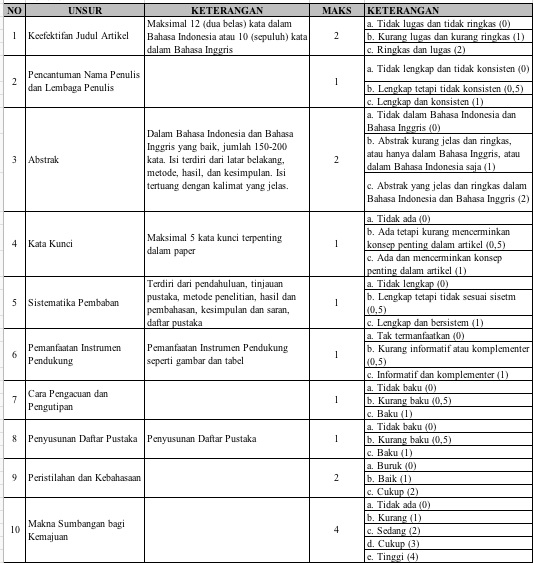
\includegraphics[width=1\textwidth]
      {figures/form1}}
      \caption{Form nilai bagian 1.}
      \label{form1}
      \end{figure}

	\begin{figure}[ht]
	      \centerline{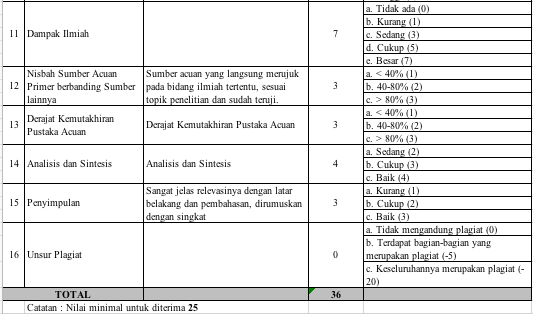
\includegraphics[width=1\textwidth]
	      {figures/form2}}
	      \caption{form nilai bagian 2.}
	      \label{form2}
	      \end{figure}

%\chapter{FAQ}

M : Kalo Intership II atau TA harus buat aplikasi ?
D : Ga harus buat aplikasi tapi harus ngoding

M : Pa saya bingung mau ngapain, saya juga bingung mau presentasi apa?
D : Makanya baca de, buka jurnal topik `ganteng' nah kamu baca dulu sehari 5 kali ya, 4 hari udah 20 tuh. Bingung itu tanda kurang wawasan alias kurang baca.

M : Pa saya sudah cari jurnal terindeks scopus tapi ga nemu.
D : Kamu punya mata de? coba dicolok dulu. Kamu udah lakuin apa aja? tolong di list laporkan ke grup Tingkat Akhir. Tinggal buka google scholar klik dari tahun 2014, cek nama jurnalnya di scimagojr.com beres.

M : Pa saya belum dapat tempat intership, jadi ga tau mau presentasi apa?
D : kamu kok ga nyambung, yang dipresentasikan itu yang kamu baca bukan yang akan kamu lakukan.

M : Pa ini jurnal harus yang terindex scopus ga bisa yang lain ?
D : Index scopus menandakan artikel tersebut dalam standar semantik yang mudah dipahami dan dibaca serta bukan artikel asal jadi. Jika diluar scopus biasanya lebih sukar untuk dibaca dan dipahami karena tidak adanya proses review yang baik dan benar terhadap artikel.

M : Pa saya tidak mengerti
D : Coba lihat standar alasan

M : Pa saya bingung
D : Coba lihat standar alasan

M : Pa saya sibuk
D : Mbahmu....

M : Pa saya ganteng
D : Ndasmu....

M : Pa saya kece
D : wes karepmu lah....


Biasanya anda memiliki alasan tertentu jika menghadapi kendala saat proses bimbingan, disini saya akan melakukan standar alasan agar persepsi yang diterima sama dan tidak salah kaprah. Penggunaan kata alasan tersebut antara lain :

1. Tidak Mengerti : anda boleh menggunakan alasan ini jika anda sudah melakukan tahapan membaca dan meresumekan 15 jurnal. Sudah mencoba dan mempraktekkan teorinya dengan mencari di youtube dan google minimal 6 jam sehari selama 3 hari berturut-turut.

2. Bingung : anda boleh mengatakan alasan bingung setelah maksimal dalam berusaha menyelesaikan tugas bimbingan dari dosen(sudah dilakukan semua). Anda belum bisa mengatakan alasan bingung jika anda masih belum menyelesaikan tugas bimbingan dan poin nomor 1 diatas. Setelah anda menyelesaikan tugas bimbingan secara maksimal dan tahap 1 poin diatas, tapi anda masih tetap bingung maka anda boleh memakai alasan ini.

%next line adds the Bibliography to the contents page
%\addcontentsline{toc}{chapter}{Bibliography}
%uncomment next line to change bibliography name to references
%\renewcommand{\bibname}{References}
%\bibliography{references}        %use a bibtex bibliography file refs.bib
%\bibliographystyle{plain}  %use the plain bibliography style
\end{enumerate}
\end{document}

